\documentclass[12pt, openany]{book}
\usepackage[a4paper,margin=1in]{geometry}
\usepackage{amsmath, amssymb, amsthm}
\usepackage{graphicx}
\usepackage[colorlinks=true, linkcolor=black, urlcolor=black, citecolor=black]{hyperref}
\usepackage{xcolor}
\usepackage{derivative}

\graphicspath{images/}

% Define Theorem, Lemma, Definition Environments
\newtheorem{theorem}{Theorem}[section]
\newtheorem{lemma}[theorem]{Lemma}
\newtheorem{proposition}[theorem]{Proposition}
\newtheorem{corollary}[theorem]{Corollary}

\theoremstyle{definition}
\newtheorem{definition}[theorem]{Definition}
\newtheorem{example}[theorem]{Example}

\theoremstyle{remark}
\newtheorem{remark}[theorem]{Remark}

% Custom Commands
\newcommand{\R}{\mathbb{R}}
\newcommand{\N}{\mathbb{N}}
\newcommand{\Z}{\mathbb{Z}}

\title{\textbf{Linear Systems and Signals Notes}}
\author{Strahinja Marinkovic}
\date{\today}

\begin{document}

\maketitle

\tableofcontents

\chapter{Signals and Systems}
\subsection{Definitions}
\begin{definition}[Signal Energy]
\[E_x = \int_{-\infty}^{\infty} |x(t)|^2dt \]
\end{definition}

\begin{definition} [Siganl Power]
    \[P_x = lim_{T \to \infty} \frac{1}{T} \int_{-T/2}^{T/2} |x(t)|^2dt\]
\end{definition}

\begin{definition} [Time Shifting]
    \[\phi(t + T) = x(t)\]
    \[\phi(t) = x(t - T)\]
    $x(t-T)$ represents $x(t)$ time shifted by T seconds.  
\end{definition}

\section{Classification of Signals}
I felt like 330 never really laid out the these basic ideas about siganls in a good way. For example, I remember Micheal and I didn't realize that anytime a signal is said to be from convolution, it is a LTI system.
\begin{figure}[h]
    \centering
    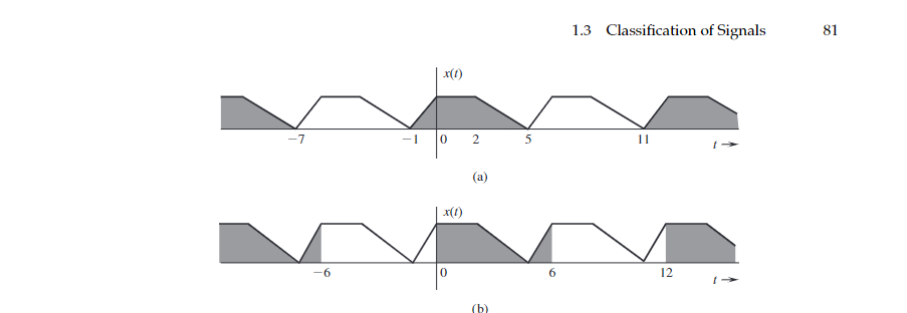
\includegraphics[width = 0.75\textwidth]{images/properties_example_1.3.png}
    \caption{Example of a property}
    \label{fig:properties_example}
\end{figure}

I like how the book goes over basic signal properites like time shifts, reversals, etc. instead of properites being introduced randomly throughout the semester (this is done well with fourier).

\begin{figure}
    \center 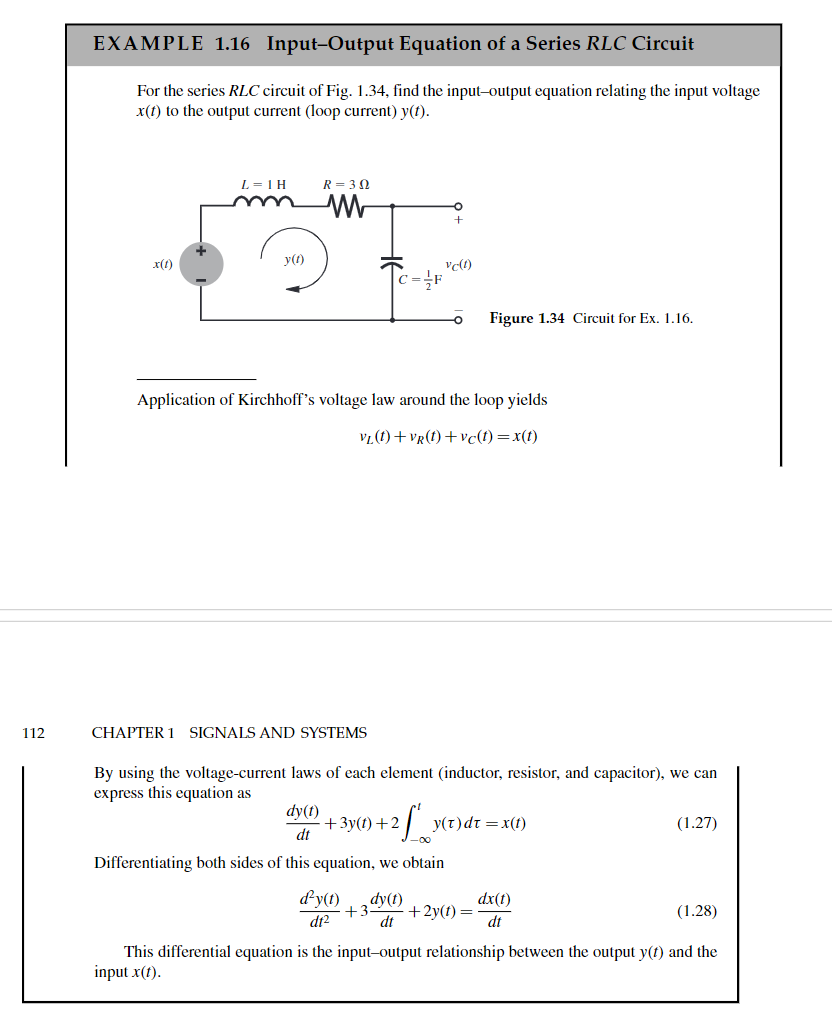
\includegraphics[width = 0.5\textwidth]{images/circuit_input_output_example.png}
\end{figure}

\begin{example} [\textbf{Unit Step Matlab Code}]
    I think students are intially confused by the idea of using the unit step function to represent other signals such as a rectangle. Might be nice to have a little matlab script.

    \begin{center}
        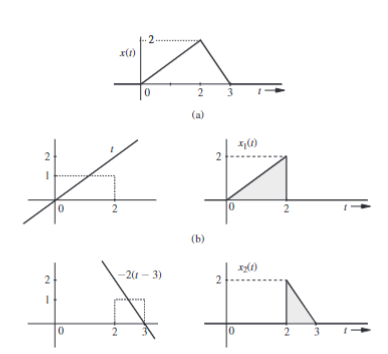
\includegraphics{images/function_w_unitstep_1.7.png}
    \end{center}
    \[x_1(t) = t[u(t) - u(t-2)]\]
    \[x_2(t) = -2(t-3)[u(t-2)-u(t-3)]\]
    \[x(t) = x_1(t) + x_2(t)\]

    Example 1.7 and drill 1.7, 1.8 are all good examples of using unit step.
\end{example}

\subsection{The Exponential Function}
\textbf{We could wait to explain this when we do Laplace.}
\subsection{Even and Odd Functions}
\textbf{Useful but seems out of place/not needed considering how much content there is to cover.}

\section{Systems}
\begin{example}
    \begin{center}
        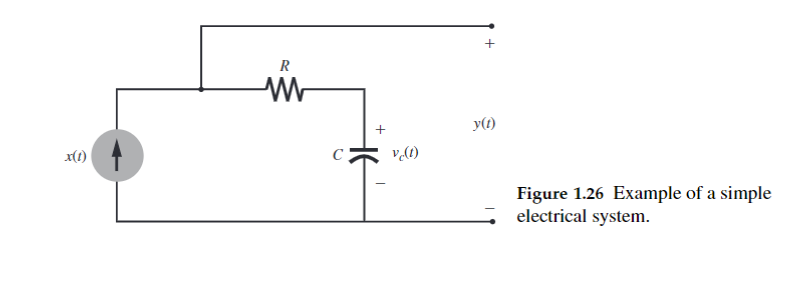
\includegraphics{images/circuits_as_system.png}
    \end{center}
    I think we should try to add a lot more circuit examples. Most students should have taken 230 by then or Physics 2.
\end{example}

\section{Classification of Systems}
Again, I think its a good idea to clearer go over all these system properties in a clear manner.

\begin{center}
    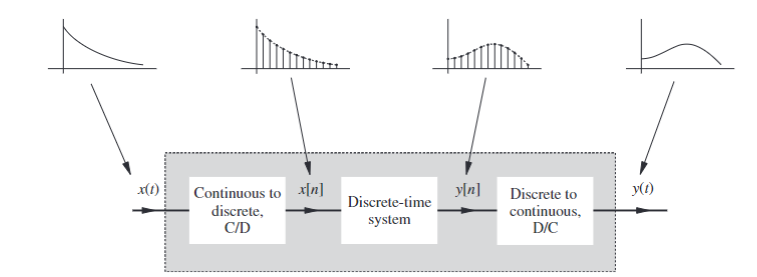
\includegraphics{images/difference_of_discrete_cont.png}
\end{center}
This is a good figure.

The end of the chapter has a lot of circuit examples that seem good.


\chapter{Time-Domain Analysis of Continuous-Time Systems}
\subsection{System Response to Internal Conditions}
What is this? We never covered zero-input response in 330.

\subsection{The Unit Impulse Response}
The book goes right into describing systems as dif. eq's. Is this the approach we want to have as well? I know before we broke down systems into a few ways: Convolution, difference equations, dif. eq, and laplace?

I personally find a complete and full derivation of something such as convolution actually helps me in my understanding and intuition. When the math is abstracted it feels like theres gaps in my understanding and like I'm missing why something is something.

The below figure demonstrates a pretty good visualization for what convolution really does. I think this was never made clear (for me) in the videos.

I want to redo the convodemo from 203 with a better GUI and make a version for continuous convolution.

I never knew until now that convolution with the unit impulse is just the function $x(t)$ itself.

The book itself has lots of good matlab examples.

What is the thought process of discrete vs continuous for teaching order? Currently 330 splits it up in terms of "operation". It first goes over convolution and then difference and differential equations. The book groups everything in terms of continuous or discrete instead.

What is easier to intuitively understand first, discrete or continuous?

Again, I really like how they format this.
\begin{itemize}
    \item Introduction
    \item Theory
    \item Example
    \item Matlab!!!
\end{itemize}

\begin{figure}
    \center 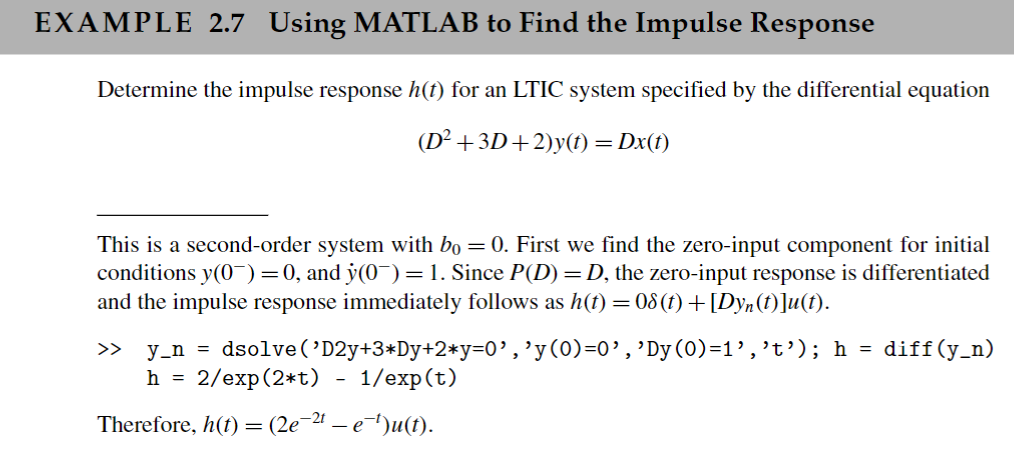
\includegraphics[width = 0.75\textwidth]{images/example 2.7.png}
\end{figure}

\begin{figure}
    \begin{center}
        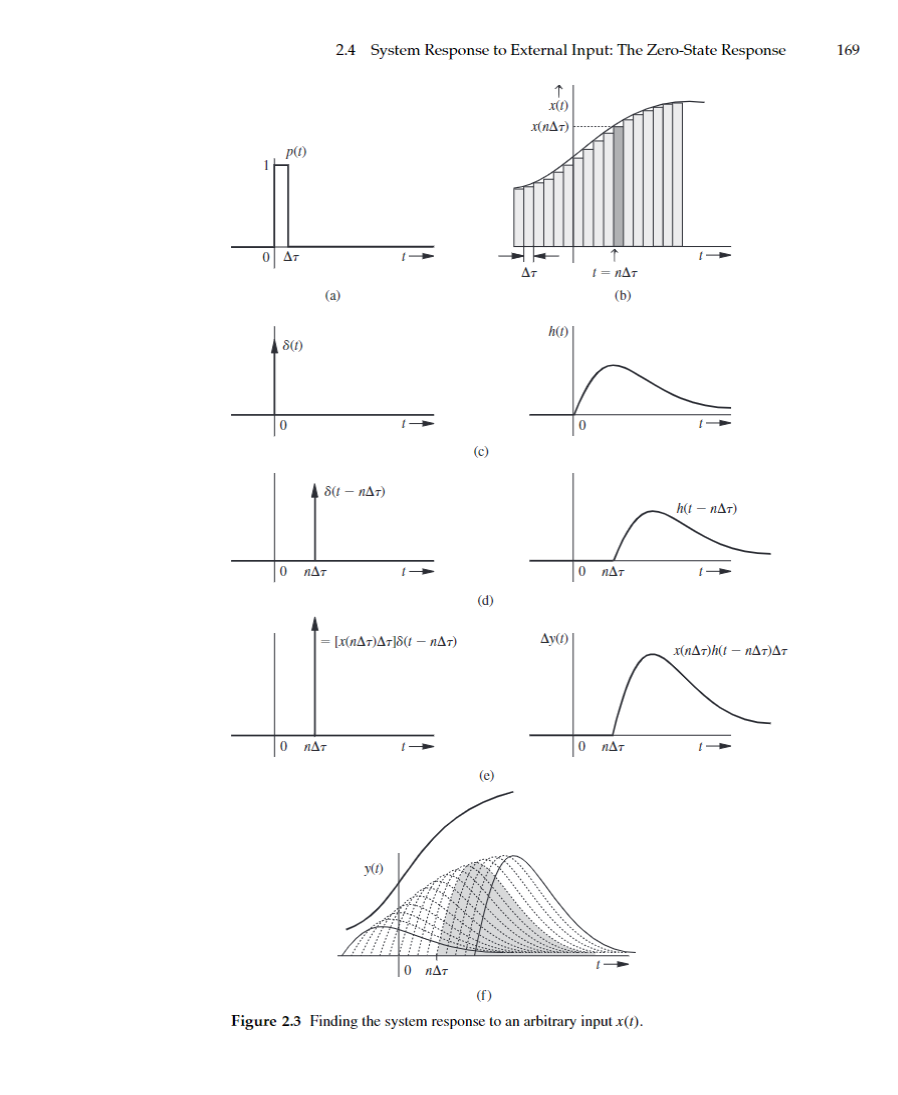
\includegraphics[width = 0.75\textwidth]{images/convolution.png}
    \end{center}
\end{figure}

\begin{figure}
    \begin{center}
       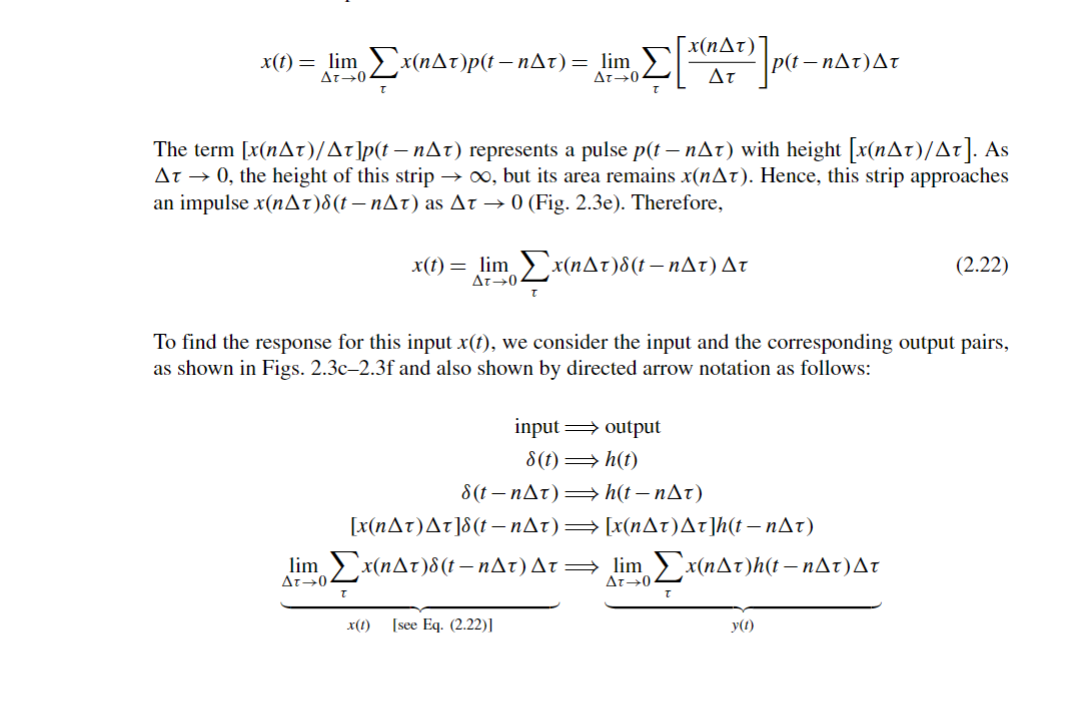
\includegraphics[width = 0.75\textwidth]{images/convolution_deriv.png}
    \end{center}
\end{figure}

\textbf{NOTE: Pg 189-190 has a good intuitive explanation of system response.}

\subsection{2.7-1 Op Amp Script Example}

KCL equation at +v(t) node
\[\frac{x(t) - v(t)}{R_3} + \frac{y(t) - v(t)}{R_2} + \frac{0-v(t)}{R_1} - C_2\odv{v}{t} = 0\]

KCL equation at inverting pin
\[\frac{v(t)}{R_1} + C_1\odv{y}{t}\]

\begin{example}
    \center
    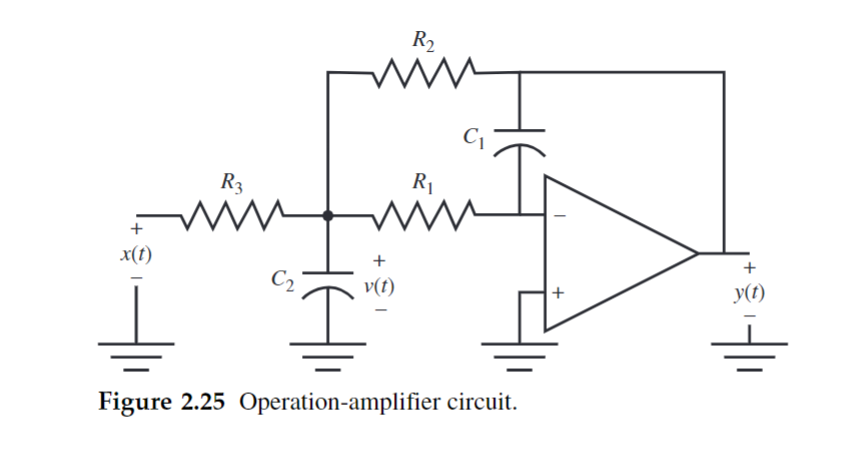
\includegraphics{images/op amp circuit.png}
\end{example}

Characteristic equation:
\[\lambda^2 + \frac{1}{C_2}{\frac{1}{R_1 + R_2 + R_3}}\lambda + \frac{1}{R_1R_2C_1C_2} = (a_0\lambda^2 + a_1\lambda + a_2) = 0\]





\chapter{Additional Notes}
\begin{itemize}

    \item We should have videos or worksheets for the math behind some of the concepts such as partial fractions, integrals, etc.
    \item Try doing more circuit examples.
    \item Keep notation consistent throughout the course...
    \item I like how the book will introduce a concept, do examples, and then give ways to visualize or solve the problems in matlab. We should try doing that more in hw's or exercises and say hey! try this yourself and mess with it.
    \item What is the order idea: Discrete vs. Continuous, what first? Or both at the same time?
\end{itemize}


\subsection{Peter's Notes}
\begin{itemize}
    \item Time invariance could be taught better with more examples. More graphical intuition.
    \item Stability was not made clear. 
    \item Have videos or text with the required math for the class (i.e. differential equations, partial fractions).
\end{itemize}

\subsection{Day by Day}

\begin{center}
    \begin{tabular}{ |c|c| } 
     \hline
     Day1 & Intro to Course + Basic Signals \\ 
     \hline
     Day2 & Impulse Function, Unit Step, Impulse response \\ 
     \hline
     Day3 & Systems + Properties \\ 
     \hline
     Day5 & Discrete Time Convolution \\ 
     \hline
     Day6 & Continuous Time Convolution \\ 
     \hline
     Day7 & Differential Equations\\ 
     \hline
     Day8 & Difference Equations \\ 
     \hline
    \end{tabular}
    \end{center}

\subsection{Student Questions/Comments}
\begin{example}
I've heard from multiple people that time invariance (and properties in general) need to be exampled a lot better considering how important they are in the course.
\begin{center}
    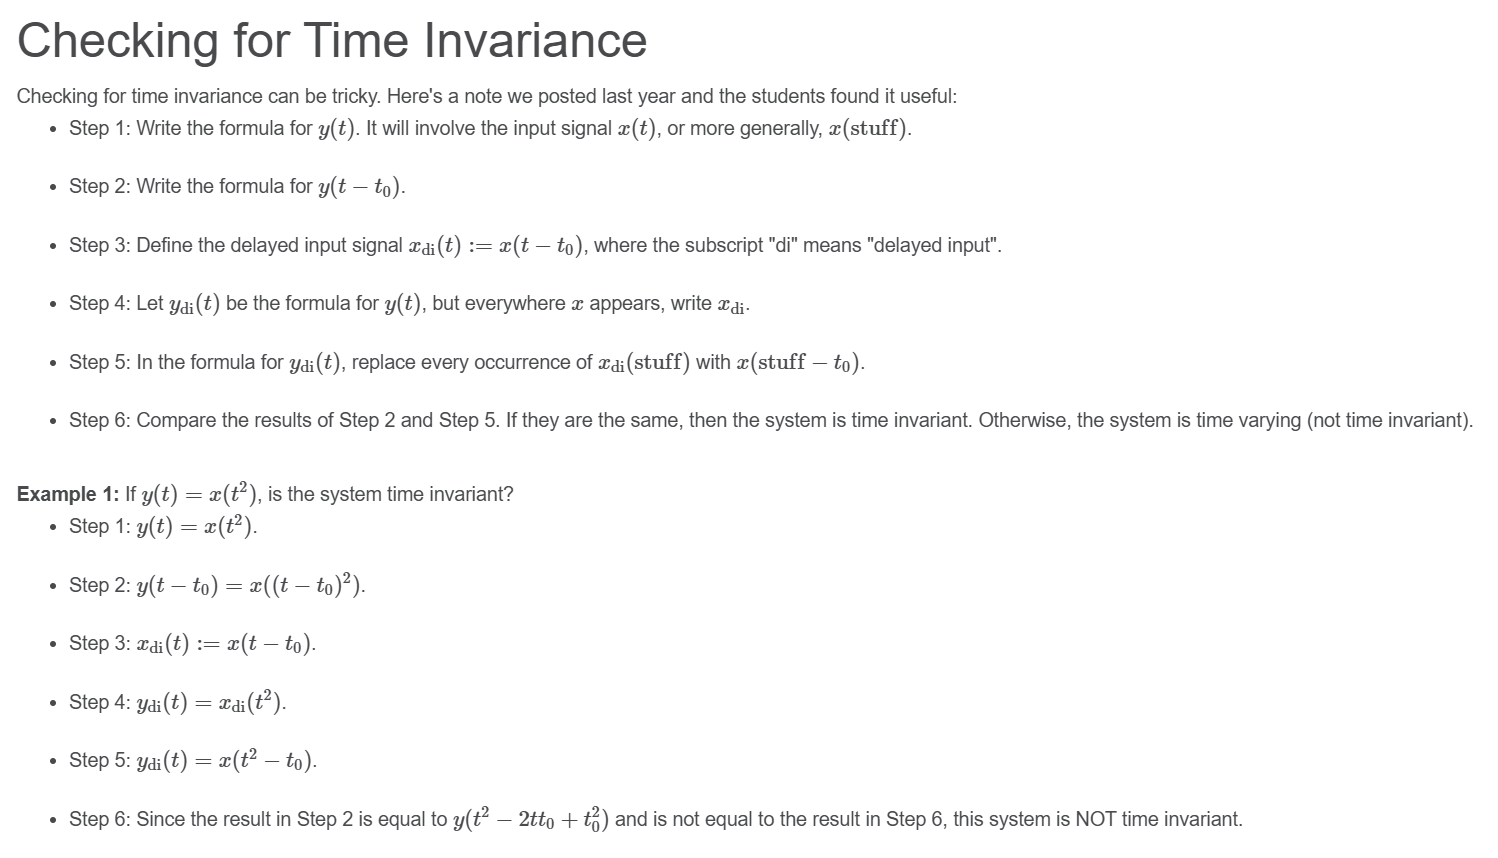
\includegraphics[width = 0.6\textwidth]{images/checking_for_time_invariance.png}       
\end{center}
\end{example}

\begin{itemize}
    \item How to know if something is BIBO stable? Considering it is the first question on the exam, it should be clear to students the steps.
    \item 
\end{itemize}



\end{document}
